\documentclass[11pt,aps,preprint,nofootinbib,superscriptaddress,tightenlines]{revtex4-2}
\usepackage[T1]{fontenc}
\usepackage{amsmath,amssymb,mathtools}
\let\lambdabar\relax   % revtex defines it; newpxmath does too
\usepackage{newpxtext,newpxmath}
\usepackage{bm}
\usepackage[final]{microtype}
\usepackage{xcolor}
\usepackage{booktabs}
\usepackage{graphicx}
\usepackage{dsfont}
\usepackage[most]{tcolorbox}
\usepackage{algpseudocode}
\newcommand{\one}{\mathds{1}}
\newcommand{\avg}[1]{\langle #1\rangle}
\newcommand{\klab}{\mathcal B}
% notation of the Density Frame paper (theory.tex)
\def\edense{{\mathcal{E}}}
\def\pdense{M}
\def\Sstress{{\mathcal S}}
\def\pr{{\mathcal P}}
\def\er{e}
\def\dd{{\rm d}}
\newcommand{\ve}[2]{e_{\;\,#1}^{#2}}
\definecolor{darkblue}{RGB}{20,60,140}
\definecolor{accent}{RGB}{30,80,150}
\definecolor{tint}{RGB}{243,246,251}
\newtcolorbox{algobox}[1]{enhanced, colback=tint, colframe=accent, boxrule=0.6pt, arc=2pt,
  left=6pt, right=6pt, top=4pt, bottom=4pt, fonttitle=\bfseries\small, coltitle=white,
  colbacktitle=accent, title={#1}, before skip=10pt, after skip=10pt}
\newtcolorbox{keyeq}{enhanced, colback=tint, frame hidden, borderline west={2pt}{0pt}{accent},
  sharp corners, left=4pt, right=4pt, top=0pt, bottom=0pt, before skip=6pt, after skip=6pt}
\usepackage[colorlinks=true,linkcolor=darkblue,citecolor=darkblue,urlcolor=darkblue]{hyperref}

\def\st{\begin{equation}}
\def\stp{\end{equation}}
\def\Eq#1{eq.~(\ref{#1})}
\def\Sect#1{Sect.~\ref{#1}}
\def\App#1{Appendix~\ref{#1}}
\def\Fig#1{Fig.~\ref{#1}}
\let\oldparagraph\paragraph
\renewcommand{\paragraph}{\par\bigskip\oldparagraph}

\begin{document}

\title{The particle model in a weak gravitational field:\\ the energy density, the pressure and the equation of state}
\author{D.~Teaney}
\affiliation{Department of Physics and Astronomy, Stony Brook University,
Stony Brook, New York 11794, USA}
\date{\today}

\begin{abstract}
The energy density and the pressure of the particle model are defined, without ambiguity, as the responses of its partition function to small changes of the
metric: the energy density to the lapse, the stress to the spatial metric.  For the particle model the responses are exact microscopic expressions, the energy of
the particles and their kinetic plus virial stress, the quantities the code measures.  With them the equation of state of the model can be measured in canonical
runs and compared with the target, with the tree-level Hamiltonian and with the renormalized one.  A lapse that varies in space spans a range of temperatures in one
run.  Driving the system out of equilibrium is outlined at the end.
\end{abstract}

\maketitle
\tableofcontents

%=============================================================================
\section{Introduction}
\label{sec:intro}

The equation of state of the particle model is not that of the fluid put in: the particles are an ideal gas of labels, and each carries the energy and the pressure
of its own fluctuations (\texttt{partition\_v2.tex}).  To check this, and to check the renormalized Hamiltonian that removes it, we need definitions of the energy
density and of the pressure of the model that are unambiguous and measurable.  Gravity provides them: the energy density is what couples to the lapse, the stress is
what couples to the spatial metric.  Small, static changes of the metric are enough; no curvature of the slices is needed.

\paragraph{Notation.}  As in the Density Frame paper \cite{densityframe} (\texttt{theory.tex}, Section ``The Metropolis algorithm in general coordinates''):
\begin{center}
\begin{tabular}{ll}
\toprule
symbol & meaning \\
\midrule
$N=e^{\sigma}$, $N^i=0$, $\gamma_{ij}=g_{ij}$ & lapse, shift and spatial metric \\
$n^\mu$, $\ve{i}{\mu}$ & normal (fiducial observer), spatial basis \\
$\edense$, $\pdense^i$, $\Sstress^{ij}$ & fiducial energy, momentum, stress densities \\
$\er(T)$, $\pr(T)$, $s(T)$ & rest-frame energy density, pressure, entropy density \\
$P^\mu=E\,n^\mu+p^i\,\ve{i}{\mu}$ & four-momentum of a particle \\
\bottomrule
\end{tabular}
\end{center}
The lapse is $N$; the number of particles is $N_p$, with mean density $\bar n=N_p/L^d$.  Particle $a$ has the position $\bm x_a$, the entropy $s_a$, the energy $E_a$ and
the momentum $p_a^i$ measured by the fiducial observer, the velocity $v_a^i=\partial E_a/\partial p_{a,i}$, and the volume $V_a=1/n_a$.  $T$ is the bare temperature at
rest, and $\sigma_{\rm p}=\pr\bar V/T$ the fluid's pressure in one particle volume over $T$ (written $\sigma$ in \texttt{partition\_v2.tex}).

%=============================================================================
\section{The background}
\label{sec:background}

We use a static metric without shift,
\begin{keyeq}
\st
\dd s^2=-e^{2\sigma(\bm x)}\,\dd t^2+g_{ij}(\bm x)\,\dd x^i\dd x^j,\qquad |\sigma|\ll1,\qquad |g_{ij}-\delta_{ij}|\ll1 ,
\label{metric}
\stp
\end{keyeq}
the Kaluza--Klein form of Jensen \emph{et al.}\ \cite{Jensen:2012jh} with no Kaluza--Klein field, and in the language of the $3+1$ split a lapse $N=e^\sigma$ and a spatial
metric $\gamma_{ij}=g_{ij}$.  Both vary slowly, on scales long compared with the kernel size $h$.  The extrinsic curvature of the slices vanishes, $K_{ij}=0$.

The lapse sets the rate of the clocks, $\dd\tau=N\,\dd t$, and is the Newtonian potential: a slow particle falls with $\ddot{\bm x}\simeq-\nabla\sigma$.  A uniform change of
the spatial metric changes the proper volume of the box at fixed coordinates, $\sqrt g\,L^d$.  With $g_{ij}=\delta_{ij}$ the conservation laws of the Density Frame
paper reduce to
\st
\partial_t\big(N\edense\big)+\partial_i\big(N^2\pdense^i\big)=0,\qquad
\partial_t\pdense^i+\partial_j\big(N\Sstress^{ij}\big)+\edense\,\partial_iN=0 :
\label{conservation}
\stp
the Killing energy $N\edense$ is conserved, and gravity pulls on the energy density.

%=============================================================================
\section{The particle model on the background}
\label{sec:model}

The generator of the time translations of a static spacetime is the Killing energy, so the particle model on the background has the Hamiltonian
\begin{keyeq}
\st
H[\sigma,g]=\sum_ae^{\sigma(\bm x_a)}\,E_a\big(s_a,\ |\bm p_a|_g,\ V_a\big),\qquad |\bm p|_g^2=g^{ij}p_ip_j ,
\label{H}
\stp
\end{keyeq}
with $E_a$ the flat-space energy of a particle, and the volume from the kernel density at proper distances,
\st
V_a=\frac1{n_a},\qquad n_a=\sum_bW\big(|\bm x_a-\bm x_b|_g\big),\qquad |\bm r|_g^2=g_{ij}r^ir^j .
\stp
The positions $x^i$ and the momenta $p_i$ are a canonical pair, so the Liouville measure $\prod_a\dd^dx_a\,\dd^dp_a\,\dd s_a$ does not depend on the metric, and the
canonical ensemble at the temperature $T_0$ is
\st
\mathcal Z_{N_p}[\sigma,g]=\frac1{N_p!}\int\prod_a\dd^dx_a\,\dd^dp_a\,\dd s_a\;\exp\Big[\sum_as_a-\frac{H[\sigma,g]}{T_0}\Big] .
\label{Z}
\stp
Hamilton's equations give $\dot{\bm x}_a=N_a\bm v_a$, the geodesic coordinate velocity, and the force $-E_a\nabla N$ plus the pressure forces weighted by the lapse, the
discrete form of \Eq{conservation}.  The stochastic step, at fixed positions and energies, keeps $H$ fixed; its time is the proper time $N_a\Delta t$.

%=============================================================================
\section{The energy density and the stress}
\label{sec:defs}

\paragraph{Definitions.}  The energy density and the stress of the model are the responses of $\ln\mathcal Z$ to the lapse and to the spatial metric,
\begin{keyeq}
\st
E(\bm x)\equiv-T(\bm x)\,\frac{\delta\ln\mathcal Z}{\delta\sigma(\bm x)},\qquad
\Sstress^{ij}(\bm x)\equiv\frac{2T(\bm x)}{\sqrt g}\,\frac{\delta\ln\mathcal Z}{\delta g_{ij}(\bm x)},\qquad T(\bm x)=T_0\,e^{-\sigma(\bm x)} ,
\label{defs}
\stp
\end{keyeq}
evaluated at the flat background.  This is the standard definition of the stress tensor as the response to the metric, applied to the equilibrium
partition function \cite{Jensen:2012jh,Banerjee:2012iz}.  The pressure is $\pr_{\rm model}=\Sstress^{ii}/d$.

\paragraph{The energy density.}  Only $H$ depends on $\sigma$, so
\begin{keyeq}
\st
E(\bm x)=\Big\langle\sum_aE_a\,\delta(\bm x-\bm x_a)\Big\rangle ,
\label{Eop}
\stp
\end{keyeq}
the energy of the particles measured by the fiducial observer, their rest energy and the kinetic energy of their momenta.

\paragraph{The stress.}  Only $H$ depends on $g_{ij}$, through the momenta and through the distances in the kernel, $\partial\ln\mathcal Z/\partial g_{ij}=-\avg{\partial H/\partial g_{ij}}/T_0$.
At $g=\delta$,
\st
\frac{\partial E_a}{\partial g_{ij}}\Big|_{\bm p}=-\tfrac12\,v_a^i\,p_a^j,\qquad
\frac{\partial E_a}{\partial g_{ij}}\Big|_{V}=\frac{\partial E_a}{\partial V_a}\,\frac{\partial V_a}{\partial g_{ij}}=-\tfrac12\,\pr_aV_a^2\,Q_a^{ij},
\stp
with $\pr_a=-\partial E_a/\partial V_a$ the mechanical pressure of a particle and
\st
Q_a^{ij}=\sum_br_{ab}^i\,D_{ab}^j,\qquad D_{ab}=-W'(r_{ab})\,\hat{\bm r}_{ab},\qquad Q_a^{ii}\simeq d\,n_a ,
\stp
the anisotropy of the star of neighbours of $a$, whose trace is $d\,n_a$ for a dense neighbourhood.  For a uniform metric change, then,
\begin{keyeq}
\st
\Sstress^{ij}=\frac1{L^d}\Big\langle\sum_a\Big(v_a^i\,p_a^j+\pr_aV_a^2\,Q_a^{ij}\Big)\Big\rangle ,
\label{Sop}
\stp
\end{keyeq}
the kinetic stress plus the virial stress, the per-particle stress $V_aT_a^{ij}=v_a^ip_a^j+\pr_aV_a^2Q_a^{ij}$ that the code measures (\texttt{statics.tex}, ``The stress
of a particle'').  Its trace over $d$ is the mechanical pressure,
\st
\pr_{\rm model}=\frac1{dL^d}\Big\langle\sum_a\Big(\bm v_a\cdot\bm p_a+\pr_aV_a^2\,Q_a^{ii}\Big)\Big\rangle\simeq\bar nT+\avg{\pr_a} ,
\stp
using equipartition, $\avg{\bm v_a\cdot\bm p_a}=d\,T$, and $Q_a^{ii}\simeq dn_a$.

\paragraph{Which pressure.}  A uniform change $g_{ij}=(1+2\epsilon)\delta_{ij}$ changes the proper volume by $\delta\ln(\sqrt gL^d)=d\,\epsilon$ at fixed $N_p$, so
\st
\pr_{\rm model}=T\,\frac{\partial\ln\mathcal Z}{\partial(\sqrt gL^d)}\Big|_{T,N_p} ,
\stp
the mechanical pressure: the derivative with respect to the volume at a fixed number of particles, the one in the momentum flux.  It differs from the ``Euler''
pressure $T\ln\mathcal Z/L^d$ by the chemical potential of the labels times their density, which depends on the normalization of the measure; the metric picks the
mechanical one.  Likewise $E$ of \Eq{defs} is $T^2\partial_T\ln\mathcal Z/L^d$ at fixed volume.

\subsection{The pressure of a particle: a Legendre transform at tree level, an average exactly}
\label{sec:particlepressure}

The stress \Eq{Sop} contains, particle by particle, the mechanical pressure of a particle, a function of its microcanonical variables,
\st
\pr_a(s,\bm p,V)=-\frac{\partial E_a}{\partial V}\Big|_{s,\bm p} .
\stp
The thermodynamics, on the other hand, gives the pressure of a particle at fixed temperature, $\pr_1(T,\bm v,V)=-\partial F_1/\partial V$, with $F_1=-T\ln Z_1$ the free
energy of one particle at fixed volume.  How are the two related?

\paragraph{At tree level: a Legendre transform.}  The tree-level free energy is the Legendre transform of the energy over the entropy and the momentum,
\st
F^{\rm tree}(T,\bm v,V)=\min_{s,\bm p}\big[E_a(s,\bm p,V)-Ts-\bm v\cdot\bm p\big] ,
\stp
and by the envelope theorem its $V$-derivative at fixed $(T,\bm v)$ is that of $E_a$ at fixed $(s,\bm p)$, at the corresponding point:
\st
\pr_1^{\rm tree}(T,\bm v,V)=\pr_a\big(s_*,\bm p_*,V\big),\qquad \frac{\partial E_a}{\partial s}\Big|_*=T,\qquad \frac{\partial E_a}{\partial\bm p}\Big|_*=\bm v ,
\stp
the familiar $(\partial E/\partial V)_S=(\partial F/\partial V)_T$.  At rest $\bm p_*=0$, $s_*=s(T)V$, and $\pr_1^{\rm tree}=\pr(T)$.

\paragraph{Exactly: an average.}  $F_1$ is an integral over the entropy and the momentum, not a maximum.  The average over one particle at fixed volume is
\st
\avg{\,\cdot\,}_{T,\bm v,V}=\frac1{Z_1}\int ds\,d^d\bm p\;(\,\cdot\,)\;e^{\,s-E_a(s,\bm p,V)/T+\bm v\cdot\bm p/T},\qquad Z_1=\int ds\,d^d\bm p\;e^{\,s-E_a/T+\bm v\cdot\bm p/T} ,
\stp
and differentiating under the integral,
\begin{keyeq}
\st
\pr_1(T,\bm v,V)=T\,\frac{\partial\ln Z_1}{\partial V}\Big|_{T,\bm v}=\avg{\pr_a}_{T,\bm v,V} .
\label{p1avg}
\stp
\end{keyeq}
This needs the measure $ds\,d^d\bm p$ and the limits of integration not to depend on $V$, which holds for the Liouville measure, flat in $s$ and $\bm p$.  A measure that
depends on $V$ breaks it: the Einstein measure, flat in $E$, carries the Jacobian $1/T_a(s,\bm p,V)$, and then $\pr_1=\avg{\pr_a}+T\avg{\partial\ln(1/T_a)/\partial V}$, a
difference of order $1/s_a$.

\paragraph{The fluctuation share.}  The average differs from the value at the saddle point by the fluctuations of the particle; at one loop, at rest,
\st
\pr_1=\pr(T)+\mathcal K_0\,\frac TV+O\Big(\frac T{Vs_a}\Big),\qquad \mathcal K_0=\frac{d+1}2 ,
\stp
the $d+1$ conserved densities of a particle each adding $T/2V$.  This is the difference between the average (a Laplace transform) and the Legendre transform; it
vanishes relative to $\pr$ as $s_a\to\infty$.

\paragraph{In the full ensemble} the volume of a particle fluctuates as well.  \Eq{p1avg} is exact conditionally, at fixed volume, and the ensemble average is
\st
\avg{\pr_a}_{\rm ens}=\big\langle\pr_1(T,V_a)\big\rangle_{V_a}\simeq\pr_1(T,\bar V)+\tfrac12\,\frac{\partial^2\pr_1}{\partial V^2}\,\avg{\delta V_a^2}+\dots ,
\stp
while the stress operator carries the factor $V_a^2Q_a^{ii}$, correlated with $V_a$.  So, from \Eq{Sop} with equipartition,
\begin{keyeq}
\st
\pr_{\rm model}=\bar nT+\avg{\pr_a}=\bar nT+\pr_1(T,\bar V)
\label{pmodel}
\stp
\end{keyeq}
holds up to the fluctuations of the volumes, which add the correction of the positions, of order $1/(\bar nh^2)$.  The measured pressure therefore contains both
one-loop pieces, the label gas $\bar nT$ (the kinetic stress) and the fluctuation share $\mathcal K_0\bar nT$, which are the pieces the renormalized Hamiltonian
removes.

%=============================================================================
\section{What to expect}
\label{sec:expect}

\paragraph{Uniform equilibrium.}  At uniform $T$ the definitions give the thermodynamics of \texttt{partition\_v2.tex}:
\st
\pr_{\rm model}=\bar nT+\pr_1(T,\bar V),\qquad E=\bar n\,\avg{E_a}_{\bar V} ,
\stp
with $\pr_1=\avg{\pr_a}$ the pressure of one particle at fixed volume (\Sect{sec:particlepressure}), plus the correction of the positions, of order $1/(\bar nh^2)$.

\paragraph{Tree-level and renormalized.}  For the conformal fluid in $d=2$, at one loop in the entropy per particle:
\begin{center}
\begin{tabular}{lcc}
\toprule
 & $\pr_{\rm model}$ & $E$ \\
\midrule
tree-level Hamiltonian & $\pr(T)+\tfrac52\,\bar nT$ & $\er(T)+5\,\bar nT$ \\
renormalized Hamiltonian ($\klab=0$) & $\pr(T)$ & $\er(T)$ \\
\bottomrule
\end{tabular}
\end{center}
Relative to the target, the tree-level terms are $2.5/\sigma_{\rm p}$ for both.  The correction of the positions adds to both Hamiltonians (\texttt{partition\_v2.tex},
``The positions back in the thermodynamics'').  At $h/a=2$ ($\bar nh^2=4.62$), with Wendland C2:
\begin{center}
\begin{tabular}{ccccc}
\toprule
 & \multicolumn{2}{c}{tree level} & \multicolumn{2}{c}{renormalized} \\
$\sigma_{\rm p}$ & $\pr_{\rm model}/\pr-1$ & $E/\er-1$ & $\pr_{\rm model}/\pr-1$ & $E/\er-1$ \\
\midrule
3.89 & $+0.56$ & $+0.62$ & $-0.067$ & $-0.039$ \\
16.4 & $+0.11$ & $+0.14$ & $-0.040$ & $-0.016$ \\
179  & $+0.002$ & $+0.010$ & $-0.012$ & $-0.004$ \\
\bottomrule
\end{tabular}
\end{center}
The tree-level entries are $2.5/\sigma_{\rm p}$ plus the correction of the positions; the renormalized entries are that correction alone, which falls as $1/(\bar nh^2)$.
At $\sigma_{\rm p}=3.9$ the exact single particle changes the tree-level entries by about $10\%$.  The trace $\pr_{\rm model}-E/2$ vanishes at one loop for both, and the
correction of the positions makes it $-0.11$, $-0.39$, $-1.44$ in units of $\bar nT$: the kernel is a scale.

%=============================================================================
\section{The measurement}
\label{sec:measurement}

\begin{algobox}{The equation of state of the model}
\begin{algorithmic}[1]
\State For each temperature $T$ in a scan, sample the canonical ensemble of the flat-space Hamiltonian, tree-level or renormalized (hybrid Monte Carlo).
\State Measure $E=\avg{\sum_aE_a}/L^d$, \Eq{Eop}, and $\pr_{\rm model}$, the trace of \Eq{Sop} over $d$.
\State Plot $E/\er(T)$, $\pr_{\rm model}/\pr(T)$ and $\pr_{\rm model}-E/2$ against $T$, for both Hamiltonians, against the table of \Sect{sec:expect}.
\State Repeat at two values of $h/a$ to separate the correction of the positions, $\propto1/(\bar nh^2)$, from the single-particle terms.
\end{algorithmic}
\end{algobox}

\paragraph{One run with a lapse.}  A lapse that varies in space, $\sigma(\bm x)=\Phi_0\cos(2\pi x/L)$, puts each particle in a local bath at the Tolman temperature
$T_0e^{-\sigma(\bm x_a)}$: the weight of \Eq{Z} is $\prod_a\exp[s_a-E_a/T(\bm x_a)]$.  Binned in slabs of constant $\sigma$, $E(\bm x)$ and the stress \Eq{Sop} give the
equation of state at the temperatures $T_0e^{\mp\Phi_0}$ in one run, and test the hydrostatic equation of the model,
\st
\nabla\pr_{\rm model}=-\big(E+\pr_{\rm model}\big)\,\nabla\sigma .
\stp
The density of particles is a second diagnostic.  The model conserves the number of particles, and in the field they redistribute so that the chemical potential of the
labels over the temperature is uniform.  With the tree-level Hamiltonian this pulls them downhill, $\bar n\propto e^{-d\sigma}$ for the conformal fluid; with the
renormalized one, whose $\mu/T$ does not depend on $T$, they stay uniform.  The field must be weak enough that $T$ varies little across a kernel and strong enough that
the variation across the box is measurable; gradients enter at relative order $(h\nabla\sigma)^2$.

%=============================================================================
\section{Measurement plan: flat space first}
\label{sec:plan}

No field is needed to test the renormalization: in flat space, $\sigma=0$ and $g_{ij}=\delta_{ij}$, the definitions \Eq{defs} give the operators \Eq{Eop} and \Eq{Sop}, and
the canonical ensemble at a known temperature gives the equation of state of the model directly.  A static metric comes later.

\paragraph{The code.}
\begin{enumerate}
\item \emph{The measurement}: a function returning, for a configuration, the energy density $\sum_aE_a/L^d$ and the stress \Eq{Sop}, its trace over $d$ the mechanical pressure,
  with the kinetic and virial parts separately.
\item \emph{The renormalized Hamiltonian} as an option, off by default: the energy of each particle evaluated at the shifted entropy
  \st
  u_a=s_a+\Delta s_a,\qquad \Delta s_a=\tfrac52\ln s_a+1+c_\chi\qquad(d=2,\ \klab=0),
  \stp
  with the temperature, the forces and the entropy function of the stochastic step all following from the same $H$ (\nolinkurl{partition_v2.tex}, ``A Hamiltonian that
  does it'').  With the option off the regression against \texttt{main} must be bit-identical.
\end{enumerate}

\paragraph{The runs.}  Canonical ensembles (hybrid Monte Carlo) at the three temperatures of the existing runs, $\sigma_{\rm p}=3.89$, $16.4$, $179$, at $h/a=2$ and $3$, with
the tree-level and the renormalized Hamiltonian: twelve runs, on the scale of the nine runs of \texttt{partition.tex}.

\paragraph{The comparison.}  $E/\er(T)-1$, $\pr_{\rm model}/\pr(T)-1$ and $\pr_{\rm model}-E/2$ against the table of \Sect{sec:expect}; the two values of $h/a$ separate the
correction of the positions ($\propto1/\bar nh^2$) from the single-particle terms.  With the renormalized Hamiltonian, also $S(k)$, which should rise at small $k$ towards
$1/\delta\klab$ (\nolinkurl{partition_v2.tex}, ``The positions back in the thermodynamics'').

%=============================================================================
\section{Results}
\label{sec:results}

Campaign \texttt{eos\_renorm} (NERSC jobs 61748587, 61751343, 61751345, \texttt{nersc/LOG.md}); figures and \texttt{docs/figs/eos\_table.csv} from
\texttt{examples/eos\_measure.py}.  Complete: both Hamiltonians at the lattice starts $s_a=16$, $54$, $541$ and $h/a=2$, $3$, $4$ in the box $L=9h$, sixteen seeds of
400 hybrid Monte Carlo updates each (one third discarded); the runs at $s_a\times0.9$, $1.1$ at $h/a=2$ for finite differences; and the boxes $L=18h$ at $h/a=2$, $3$
for $S(k)$, eight seeds each.  The statistical errors of $E/\er-1$ and $\pr_{\rm model}/\pr-1$ are $1$--$5\times10^{-4}$ (between seeds).  Extension: the boxes
$L=36h$ at $h/a=2$ ($N=6048$, sixteen seeds each) for $S(k)$ at small $k$ (job 61762047).  The renormalized Hamiltonian shifts the temperature of a lattice start, so its $\sigma_{\rm p}$ are $5.16$, $18.0$ and
$180$ in place of $3.89$, $16.4$ and $179$.

\paragraph{The predictions at $\sigma_{\rm p}=3.89$.}  At this small entropy per particle the one-loop values are not enough, and the exact single particle
(quadrature of $F_1$, \texttt{partition.tex}, ``Small entropy per particle'') gives $\Pi-\sigma_{\rm p}=1.35$ in place of $\mathcal K_0=3/2$ and $\Delta e=4.7\,T$ in place of $5\,T$.
With the correction of the positions at $h/a=2$ ($\delta p=-0.32\,\bar nT$, $\delta e_a=-0.20\,T$, \texttt{partition\_v2.tex}),
\st
\frac{\pr_{\rm model}}{\pr}-1=\frac{1+(\Pi-\sigma_{\rm p})+\delta p/\bar nT}{\sigma_{\rm p}},\qquad
\frac{E}{\er}-1=\frac{\Delta e/T+\delta e_a/T}{2\sigma_{\rm p}} .
\stp

\begin{center}
\begin{tabular}{lccc}
\toprule
quantity & one loop & exact single particle $+$ positions & measured (tree level) \\
\midrule
$E/\er(T_0)-1$ & $0.643$ & $0.578$ & $0.5762\pm0.0005$ \\
$\pr_{\rm model}/\pr(T_0)-1$ & $0.643$ & $0.522$ & $0.5203\pm0.0005$ \\
kinetic stress $/\bar nT$ & $1$ & $1$ & $1.0001\pm0.0007$ \\
(virial $-\pr$)$/\bar nT$ & $1.5$ & $1.03$ & $1.026\pm0.002$ \\
$(\pr_{\rm model}-E/2)/\bar nT$ & $0$ & $-0.22$ & $-0.2179\pm0.0004$ \\
$(\partial E/\partial T)/(de/dT)-1$ & $0.214$ & & $0.21\pm0.03$ \\
$(\partial\pr/\partial T)/(dp/dT)-1$ & $0.214$ & & $0.17\pm0.03$ \\
$c_s^2$ at fixed $\bar n$ & $0.5$ & & $0.4837\pm0.0014$ \\
\bottomrule
\end{tabular}
\end{center}
At $h/a=3$ and $4$ the two entries rise to $0.593$, $0.598$ ($E$) and $0.568$, $0.584$ ($\pr_{\rm model}$); linear in $1/(\bar nh^2)$ both extrapolate to $0.604$, which is
the exact single particle alone, $(1+1.35)/3.89=4.7/(2\times3.89)=0.604$.

\paragraph{The equation of state at $\sigma_{\rm p}=16$--$180$.}  Against \Sect{sec:expect}: the predictions (in brackets) are the table there at $h/a=2$, with the
correction of the positions scaled by $4.62/(\bar nh^2)$ at $h/a=3$, $4$ ($\bar nh^2=10.4$, $18.5$); for the renormalized runs, the entries at $\sigma_{\rm p}=16.4$ and
$179$.  Trace in units of $\bar nT$.
\begin{center}
\small
\begin{tabular}{lcccccc}
\toprule
 & $\sigma_{\rm p}$ & $h/a$ & $E/\er-1$ & $\pr_{\rm model}/\pr-1$ & $(\pr_{\rm model}-E/2)/\bar nT$ & $\times\,\bar nh^2$ \\
\midrule
tree & 16.4 & 2 & $+0.135$ ($+$0.140) & $+0.107$ ($+$0.110) & $-0.463$ ($-$0.390) & $-2.14$ \\
tree & 16.4 & 3 & $+0.144$ ($+$0.147) & $+0.131$ ($+$0.134) & $-0.202$ ($-$0.173) & $-2.09$ \\
tree & 16.4 & 4 & $+0.147$ ($+$0.149) & $+0.140$ ($+$0.142) & $-0.113$ ($-$0.098) & $-2.08$ \\
tree & 179 & 2 & $+0.0099$ ($+$0.0100) & $+0.0009$ ($+$0.0020) & $-1.595$ ($-$1.440) & $-7.37$ \\
tree & 179 & 3 & $+0.0123$ ($+$0.0122) & $+0.0086$ ($+$0.0086) & $-0.671$ ($-$0.640) & $-6.97$ \\
tree & 179 & 4 & $+0.0130$ ($+$0.0130) & $+0.0109$ ($+$0.0110) & $-0.371$ ($-$0.360) & $-6.85$ \\
renorm. & 18 & 2 & $-0.015$ ($-$0.016) & $-0.039$ ($-$0.040) & $-0.437$ ($-$0.390) & $-2.02$ \\
renorm. & 18 & 3 & $-0.006$ ($-$0.007) & $-0.017$ ($-$0.018) & $-0.190$ ($-$0.173) & $-1.97$ \\
renorm. & 18 & 4 & $-0.003$ ($-$0.004) & $-0.009$ ($-$0.010) & $-0.106$ ($-$0.098) & $-1.96$ \\
renorm. & 180 & 2 & $-0.0041$ ($-$0.0040) & $-0.0129$ ($-$0.0120) & $-1.588$ ($-$1.440) & $-7.33$ \\
renorm. & 180 & 3 & $-0.0017$ ($-$0.0018) & $-0.0054$ ($-$0.0053) & $-0.668$ ($-$0.640) & $-6.95$ \\
renorm. & 180 & 4 & $-0.0009$ ($-$0.0010) & $-0.0030$ ($-$0.0030) & $-0.370$ ($-$0.360) & $-6.83$ \\
\bottomrule
\end{tabular}
\end{center}

\paragraph{Temperature derivatives: finite differences.}  The runs at $s_a\times0.9$ and $1.1$ have the same lattice, hence the same density, at temperatures $\pm5\%$ apart;
$\partial E/\partial T\simeq\Delta E/\Delta T$ and $c_s^2=\Delta\pr_{\rm model}/\Delta E$ at fixed $\bar n$ are fifteen times more precise than the canonical fluctuations
(\Fig{fig:derivs}, in brackets), with which they agree.  At fixed density $\sigma_{\rm p}\propto T^2$, so a term $c/\sigma_{\rm p}$ in $E/\er-1$ adds $c/(3\sigma_{\rm p})$ to
$(\partial E/\partial T)/(d\er/dT)-1$: the one-loop $5/(6\sigma_{\rm p})$ at tree level.
\begin{center}
\small
\resizebox{\textwidth}{!}{\begin{tabular}{lcccc}
\toprule
 & $\sigma_{\rm p}$ & $(\partial E/\partial T)/(d\er/dT)-1$ & $(\partial\pr_{\rm model}/\partial T)/(d\pr/dT)-1$ & $c_s^2$ at fixed $\bar n$ \\
\midrule
tree & 16.4 & $+0.042\pm0.001$ ($+0.07\pm0.02$) & $+0.023\pm0.001$ ($+0.05\pm0.02$) & $0.4906\pm0.0008$ ($0.4900\pm0.0013$) \\
tree & 179 & $+0.0004\pm0.0003$ ($-0.03\pm0.02$) & $-0.0056\pm0.0003$ ($-0.04\pm0.02$) & $0.4970\pm0.0002$ ($0.4963\pm0.0008$) \\
renorm. & 18.0 & $-0.011\pm0.001$ ($-0.03\pm0.02$) & $-0.030\pm0.001$ ($-0.05\pm0.02$) & $0.4906\pm0.0009$ ($0.4892\pm0.0010$) \\
renorm. & 180 & $-0.0043\pm0.0003$ ($-0.02\pm0.02$) & $-0.0102\pm0.0003$ ($-0.02\pm0.02$) & $0.4970\pm0.0002$ ($0.4964\pm0.0005$) \\
\bottomrule
\end{tabular}}
\end{center}

\paragraph{What it shows.}
\begin{itemize}
\item \emph{The renormalization works.}  The renormalized Hamiltonian removes the tree-level excess $2.5/\sigma_{\rm p}$ (\Fig{fig:EP}): what remains is the correction of the
  positions, as predicted to $10\%$ or better at $\sigma_{\rm p}=18$ and $180$ and every $h/a$, and it falls as $1/(\bar nh^2)$ (at $\sigma_{\rm p}=18$,
  $\bar nh^2(\pr_{\rm model}/\pr-1)=-0.180$, $-0.172$, $-0.161$ at $h/a=2$, $3$, $4$).
\item The tree-level entries are $2.5/\sigma_{\rm p}$ plus the same correction, to $\pm0.005$ at $\sigma_{\rm p}=16.4$ and $\pm0.001$ at $179$.  At $\sigma_{\rm p}=3.9$ the
  exact single particle is needed (above).
\item The kinetic stress is $\bar nT$ to $0.1\%$ in every run (equipartition).
\item \emph{The trace is the positions'.}  $\pr_{\rm model}-E/2$ is nearly the same for both Hamiltonians ($6\%$ at $\sigma_{\rm p}\approx17$, $1\%$ at $180$), and $\bar nh^2(\pr_{\rm model}-E/2)/\bar nT$ collapses across
  $h/a$ (\Fig{fig:trace}): $-2.0$ to $-2.1$ at $\sigma_{\rm p}\approx17$, $-6.8$ to $-7.4$ at $\sigma_{\rm p}\approx180$.  It is larger than the one-loop
  correction of the positions ($-1.80$, $-6.65$), by $9$--$19\%$ at $\sigma_{\rm p}\approx17$ and $3$--$11\%$ at $180$, most at $h/a=2$: the next order in $1/(\bar nh^2)$.
\item \emph{So is the departure of $c_s^2$ from $1/2$.}  The finite differences give the same $c_s^2$ for both Hamiltonians, $0.4906$ at $\sigma_{\rm p}\approx17$ and $0.4970$ at
  $180$, and the fluctuation values approach $1/2$ as $1/(\bar nh^2)$ ($1/2-c_s^2=0.016$, $0.007$, $0.005$ at $s_a=16$, $h/a=2$, $3$, $4$, tree level): the labels
  contribute nothing to it, the kernel does.  The slopes are additive: the tree-level $+0.042$ at $\sigma_{\rm p}=16.4$ is the one-loop $5/(6\sigma_{\rm p})=0.051$ plus the
  positions' $-0.011$ (the renormalized value).
\item \emph{Renormalized at small entropy per particle} ($s_a=16$, $\sigma_{\rm p}=5.16$): $E/\er-1=+0.026$, $+0.038$, $+0.042$ and $\pr_{\rm model}/\pr-1=-0.009$,
  $+0.023$, $+0.034$ at $h/a=2$, $3$, $4$, both extrapolating to $+0.048$ at $\bar nh^2\to\infty$, with the trace going to zero.  The one-loop counterterm leaves
  a single-particle remainder of about $0.25/\sigma_{\rm p}$ here, the counterpart of the tree level's $-0.038$ at $\sigma_{\rm p}=3.9$ (above); it is not in the
  predictions of \Sect{sec:expect}, and a quadrature of the renormalized single particle at $\sigma_{\rm p}=5.2$ would check it.  The temperature derivatives
  there, $-0.11$, $-0.07$, $-0.08$ (canonical fluctuations, $\pm0.02$), carry the same remainder.
\end{itemize}

\begin{figure}[h]
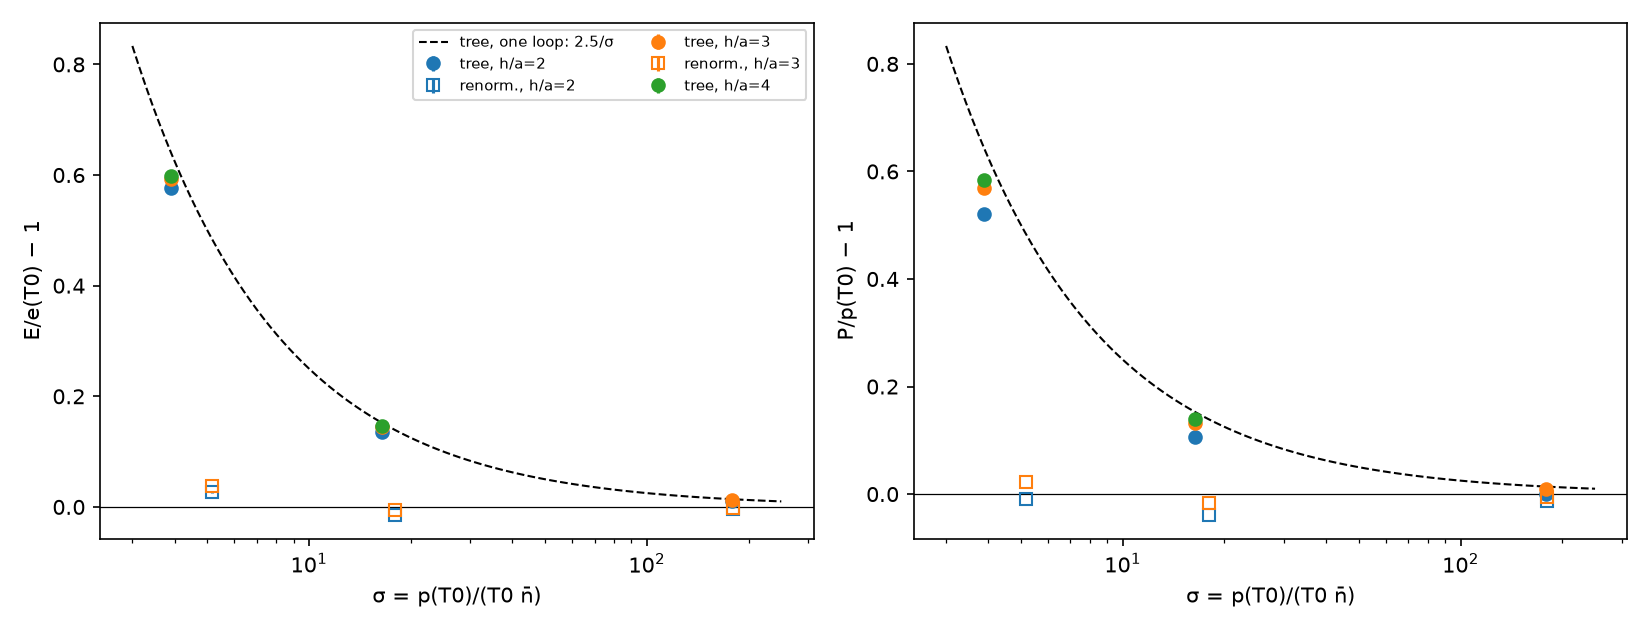
\includegraphics[width=\textwidth]{figs/eos_EP.png}
\caption{$E/\er(T_0)-1$ (left) and $\pr_{\rm model}/\pr(T_0)-1$ (right) against $\sigma_{\rm p}$; filled, tree level; open, renormalized; colours by $h/a$.  Dashed: the
one-loop tree-level value $2.5/\sigma_{\rm p}$.}
\label{fig:EP}
\end{figure}

\begin{figure}[h]
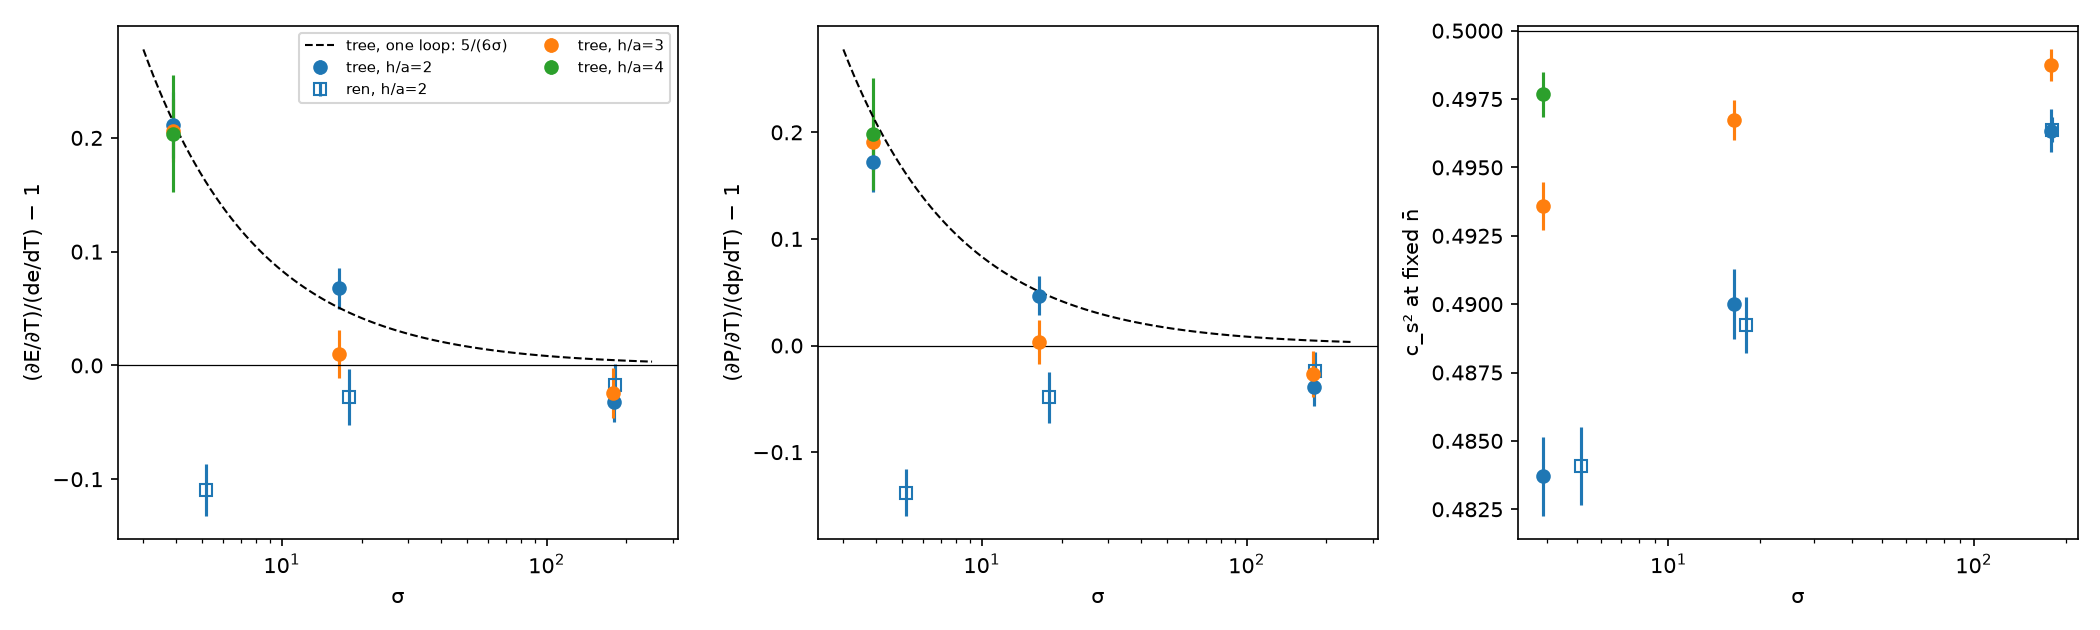
\includegraphics[width=\textwidth]{figs/eos_derivs.png}
\caption{$\partial E/\partial T$ and $\partial\pr/\partial T$ at fixed density over the target, and $c_s^2$ at fixed density, from the canonical fluctuations; black diamonds,
finite differences from the runs at $s_a\times0.9$, $1.1$ ($h/a=2$; filled, tree; open, renormalized).  Dashed: one loop, tree level.}
\label{fig:derivs}
\end{figure}

\begin{figure}[h]
\centering
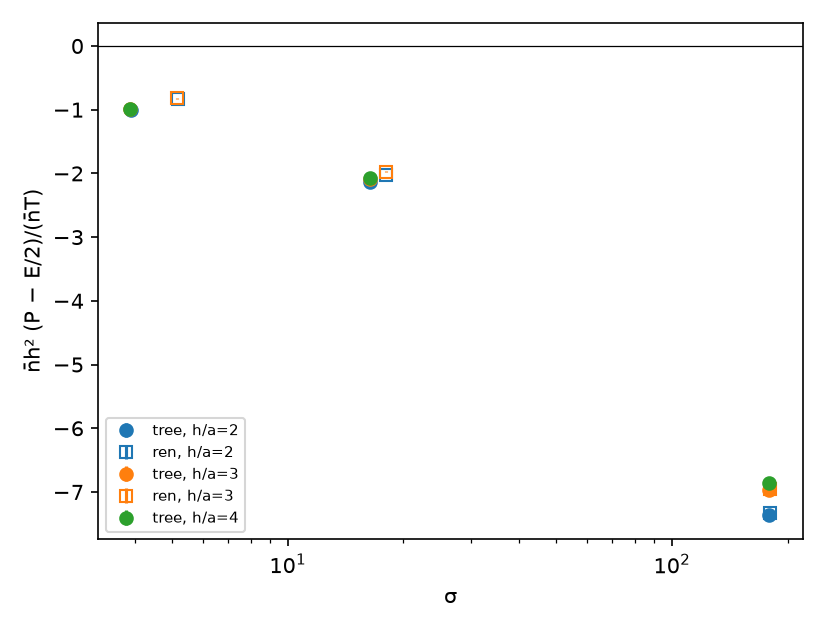
\includegraphics[width=0.55\textwidth]{figs/eos_trace.png}
\caption{The trace times the number of neighbours, $\bar nh^2(\pr_{\rm model}-E/2)/\bar nT$, which collapses the correction of the positions across $h/a$; filled, tree level; open, renormalized.}
\label{fig:trace}
\end{figure}

\paragraph{The structure factor.}  In the boxes $L=0.9=18h$ at $h/a=2$ and $3$ ($N=1512$ and $3402$, eight seeds each), $S(k)$ of the positions, averaged over shells of $|\bm k|$, against
the Ornstein--Zernike form of \texttt{partition\_v2.tex},
\st
S(k)\simeq\frac1{\klab+\delta\klab+\sigma_{\rm p}\mu_2k^2/2},\qquad \mu_2=\tfrac59h^2\ \ \text{(Wendland C2)},
\label{SkOZ}
\stp
with $\klab=5/2$ at tree level and $0$ renormalized, and $\delta\klab$ the bulk modulus supplied by the positions ($0.36$ at $\sigma_{\rm p}=16.4$, $0.95$ at $179$ for
$h/a=2$, \texttt{partition\_v2.tex}, scaled by $4.62/(\bar nh^2)$ at $h/a=3$): no free parameter.
\begin{center}
\resizebox{\textwidth}{!}{\begin{tabular}{lccccc}
\toprule
 & $\sigma_{\rm p}$ & $S(0)$ predicted & $kh=0.35$ & $kh=0.49$ & $kh=0.70$ \\
\midrule
\multicolumn{6}{l}{$h/a=2$} \\
tree, $s_a=54$ & 16.4 & 0.35 & $0.316\pm0.012$ (0.293) & $0.271\pm0.014$ (0.253) & $0.209\pm0.005$ (0.196) \\
renormalized, $s_a=54$ & 18.0 & 2.6 & $1.05\pm0.04$ (1.00) & $0.67\pm0.04$ (0.63) & $0.390\pm0.013$ (0.353) \\
tree, $s_a=541$ & 179 & 0.29 & $0.101\pm0.006$ (0.105) & $0.066\pm0.004$ (0.065) & $0.040\pm0.003$ (0.036) \\
renormalized, $s_a=541$ & 180 & 1.05 & $0.123\pm0.010$ (0.141) & $0.085\pm0.006$ (0.077) & $0.044\pm0.002$ (0.039) \\
\multicolumn{6}{l}{$h/a=2$, $L=36h$: $kh=0.175$, $0.246$, $0.35$} \\
renormalized, $s_a=54$ & 18.0 & 2.6 & $1.89\pm0.18$ (1.87) & $1.34\pm0.07$ (1.46) & $1.02\pm0.04$ (1.01) \\
tree, $s_a=541$ & 179 & 0.29 & $0.202\pm0.019$ (0.202) & $0.139\pm0.010$ (0.155) & $0.099\pm0.005$ (0.106) \\
renormalized, $s_a=541$ & 180 & 1.05 & $0.302\pm0.025$ (0.405) & $0.232\pm0.022$ (0.251) & $0.136\pm0.007$ (0.143) \\
\multicolumn{6}{l}{$h/a=3$} \\
tree, $s_a=54$ & 16.4 & 0.38 & $0.312\pm0.011$ (0.311) & $0.276\pm0.013$ (0.266) & $0.223\pm0.003$ (0.204) \\
renormalized, $s_a=54$ & 18.0 & 5.9 & $1.39\pm0.12$ (1.28) & $0.685\pm0.025$ (0.730) & $0.423\pm0.013$ (0.382) \\
tree, $s_a=541$ & 179 & 0.34 & $0.112\pm0.012$ (0.111) & $0.067\pm0.004$ (0.067) & $0.041\pm0.001$ (0.037) \\
renormalized, $s_a=541$ & 180 & 2.4 & $0.159\pm0.012$ (0.152) & $0.078\pm0.007$ (0.080) & $0.042\pm0.003$ (0.040) \\
\bottomrule
\end{tabular}}
\end{center}
(in brackets, \Eq{SkOZ}).
\begin{itemize}
\item At $s_a=54$ the renormalized $S(k)$ rises at small $k$ as predicted: three times the tree-level value at $kh=0.35$, on the curve \Eq{SkOZ} with
  $\klab=\delta\klab$ to $5\%$; at $h/a=3$, where $\delta\klab$ is smaller, it rises further ($1.39\pm0.12$, predicted $1.28$).  The labels of the renormalized Hamiltonian are neutral, and the positions are held at long wavelength only by the pressure through
  the kernel and by $\delta\klab$; the correlation length is $\xi=3.6h$ ($5.4h$ at $h/a=3$) against $1.3h$ at tree level.
\item In the boxes $L=36h$ ($kh_{\rm min}=0.175$) at $s_a=54$ the renormalized $S(k)$ continues on the curve, $1.89\pm0.18$ against $1.87$, two thirds of the way to its
  plateau $S(0)=2.6$; a fit of \Eq{SkOZ} with the $k^2$ term fixed at $kh\le0.25$ gives $\klab+\delta\klab=0.42\pm0.03$, against $\delta\klab=0.38$.
\item At $s_a=541$ the two Hamiltonians differ only below $kh\approx0.3$ ($\xi=7.3h$ against $3.8h$).  The box $L=18h$ does not reach it; in the box $L=36h$ the tree
  level is on the curve ($0.202\pm0.019$ against $0.202$ at $kh=0.175$), and the renormalized $S(k)$ rises above it, $0.30\pm0.03$, but less than predicted, $0.40$.
  The same fit gives $\klab+\delta\klab=3.8\pm0.3$ at tree level and $1.65\pm0.23$ renormalized, against $3.45$ and $0.95$: their difference, $2.2\pm0.4$, is the label
  modulus $5/2$, and the modulus supplied by the positions, $\delta\klab\approx1.6$, is above the one-loop $0.95$, as the trace is (above), by more.  So $S(0)\approx0.6$
  at $\sigma_{\rm p}=180$, $h/a=2$, and the turnover itself is below $kh\approx0.15$.
\item The tree-level $S(k)$ is below $1$ everywhere, $S(0)=1/(\klab+\delta\klab)$: the counting term holds the particles at the preferred density.
\item Above $kh\approx0.8$ the data lie above \Eq{SkOZ} by $10$--$30\%$, as expected of a small-$k$ form; the full $S(k)=1/(1+A(k))$ is not compared here.
\end{itemize}

\begin{figure}[h]
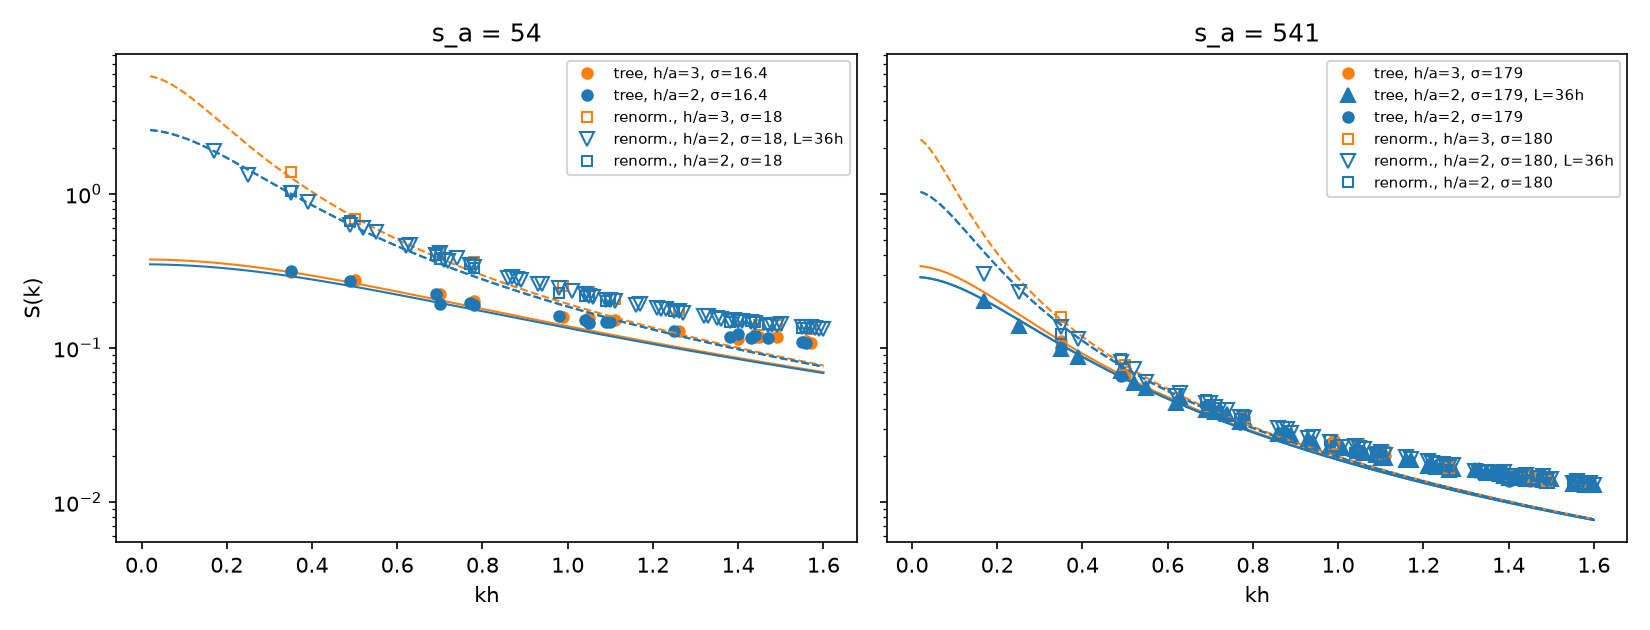
\includegraphics[width=\textwidth]{figs/eos_Sk.png}
\caption{$S(k)$ of the positions in the boxes $L=18h$ (circles, squares) and $L=36h$ (triangles), averaged over shells of $|\bm k|$; filled, tree level; open, renormalized.  Lines: Ornstein--Zernike,
\Eq{SkOZ}, with $\delta\klab$ from \texttt{partition\_v2.tex} (solid, tree level; dashed, renormalized).  Left $s_a=54$, right $s_a=541$; colours by $h/a$.}
\label{fig:Sk}
\end{figure}

%=============================================================================
\section{The equilibrium partition function as a generating functional}
\label{sec:jensen}

Jensen \emph{et al.}\ \cite{Jensen:2012jh} and Banerjee \emph{et al.}\ \cite{Banerjee:2012iz} showed that in a stationary background $\ln Z$ is a local functional of the
metric, organized in derivatives, whose variations are the equilibrium densities.  For a fluid without a conserved charge, at zeroth order,
\st
W_0[\sigma,g]=\int\dd^dx\,\sqrt g\;\frac{e^{\sigma}}{T_0}\,\pr\big(T_0e^{-\sigma}\big) ,
\stp
with Tolman's law built in, and \Eq{defs} applied to it gives $E=\er(T)$ and $\Sstress^{ij}=\pr(T)\,\delta^{ij}$.  The equation of state is the one function of the zeroth
order.  At second order, with flat slices and no shift, one more function appears, the coefficient of $(\nabla T)^2$, an equilibrium (hydrostatic) coefficient rather than
a transport coefficient; for the particle model it is generated by the kernel at order $h^2$, and a field of wavenumber $k$ measures it through corrections of relative
order $(kh)^2$.  The dissipative coefficients do not appear in $W$.

%=============================================================================
\section{Out of equilibrium: an outline}
\label{sec:outofeq}

A metric that changes in time drives the system out of equilibrium.
\begin{itemize}
\item \emph{A lapse switched on or oscillating}, $\sigma=\Phi_0\cos(kx)\cos\omega t$, drives longitudinal motion through the force $-\edense\nabla N$: sound waves, whose damping
  measures $\zeta+2(d-1)\eta/d$ ($\zeta+\eta$ in $d=2$) and whose speed is the model's along the curve of fixed entropy per particle.
\item \emph{A spatial metric oscillating in time}, $g_{ij}=\delta_{ij}+h_{ij}(t)$, strains the fluid directly.  A traceless uniform $h_{xy}(t)$ is a shear strain, whose response
  is $\Sstress^{xy}=-\pr\,h_{xy}-\eta\,\dot h_{xy}$ at low frequency: the Kubo formula for the shear viscosity, with \Eq{Sop} as the operator.  The trace part measures $\zeta$.
\end{itemize}
These are the subject of the next part.

\begin{thebibliography}{9}
\bibitem{densityframe} J.~Bhambure, R.~Singh and D.~Teaney, \emph{Stochastic relativistic viscous hydrodynamics from the Metropolis algorithm} (the Density Frame
  paper, \texttt{theory.tex}).
\bibitem{Jensen:2012jh} K.~Jensen, M.~Kaminski, P.~Kovtun, R.~Meyer, A.~Ritz and A.~Yarom, \emph{Towards hydrodynamics without an entropy current},
  Phys.\ Rev.\ Lett.\ \textbf{109}, 101601 (2012), arXiv:1203.3556.
\bibitem{Banerjee:2012iz} N.~Banerjee, J.~Bhattacharya, S.~Bhattacharyya, S.~Jain, S.~Minwalla and T.~Sharma, \emph{Constraints on fluid dynamics from equilibrium
  partition functions}, JHEP \textbf{09}, 046 (2012), arXiv:1203.3544.
\end{thebibliography}

\end{document}
